\subsubsection{模型建立}

针对问题二，先建立中心趋势决策模型，再建立固定方案的样本外评价模型。

\textbf{步骤1 中心趋势路径}

小麦和玉米销量年增长率取7.5\%，其他作物取0；亩产量保持基准水平，成本每年增长5\%，粮食价格不变，蔬菜价格每年增长5\%，一般食用菌价格每年下降3\%，羊肚菌下降5\%，各变化率按复利逐年累乘得到各年参数。设中心路径参数为$D^c_{tj}$、$y^c_{tgsj}$、$c^c_{tgsj}$和$p^c_{tgsj}$。

\textbf{步骤2 固定方案MILP}

正式方案在$\alpha=0.5$下求解
\begin{equation}
\max \Pi_c^{(0.5)}=\sum_{t,i,s,j}\Bigl\{p^c_{tg_i s j}\Bigl[0.5y^c_{tg_i s j}x_{tisj}+0.5q_{tisj}\Bigr]-c^c_{tg_i s j}x_{tisj}\Bigr\}.
\end{equation}
面积变量$x_{tisj}$不带情景索引，管理配置固定为$\rho=0.1$且每地块季次最多3种作物。

\textbf{步骤3 样本外评估}

用种子3026生成200个测试情景。小麦和玉米销量增长率在$[5\%,10\%]$内抽样，其他作物在$[-5\%,5\%]$内抽样，亩产量变化率在$[-10\%,10\%]$内抽样。固定方案在情景$\omega$下的收益为
\begin{equation}
\Pi_{\omega}^{(\alpha)}(x)=\sum_t\left[R_{t\omega}^{(\alpha)}(x)-C_{t\omega}(x)\right].
\end{equation}
最差5\%平均收益定义为
\begin{equation}
\operatorname{LTM}_{0.05}^{(\alpha)}=\frac{1}{|\Omega_{0.05}|}\sum_{\omega\in\Omega_{0.05}}\Pi_{\omega}^{(\alpha)}.
\end{equation}

\subsubsection{模型求解}

半价销售模式下，主方案平均七年净收益为6897.19万元，比基线高5.68万元，最差5\%情景平均收益为6317.80万元。将同一固定方案置于滞销模式时，平均收益为2578.45万元。两种模式的200个正式测试情景中均未出现负收益，硬约束违反数为0。

方案结构上，主方案与基线均使用24种作物，但主方案前三作物面积占比升至44.41\%（基线为42.10\%），Gini-Simpson多样性指标为0.8993，逐地块作物面积重合度仅为28.63\%。这说明中心趋势信息主要改变了地块层面的微观调度，而非作物数量或宏观结构，未造成作物种类退化。

图\ref{fig:q2_risk}显示，半价模式的平均收益优势较小，5\%分位数并未高于基线，因此不能把均值改善解释成全面下尾优势。
\begin{figure}[H]
  \centering
  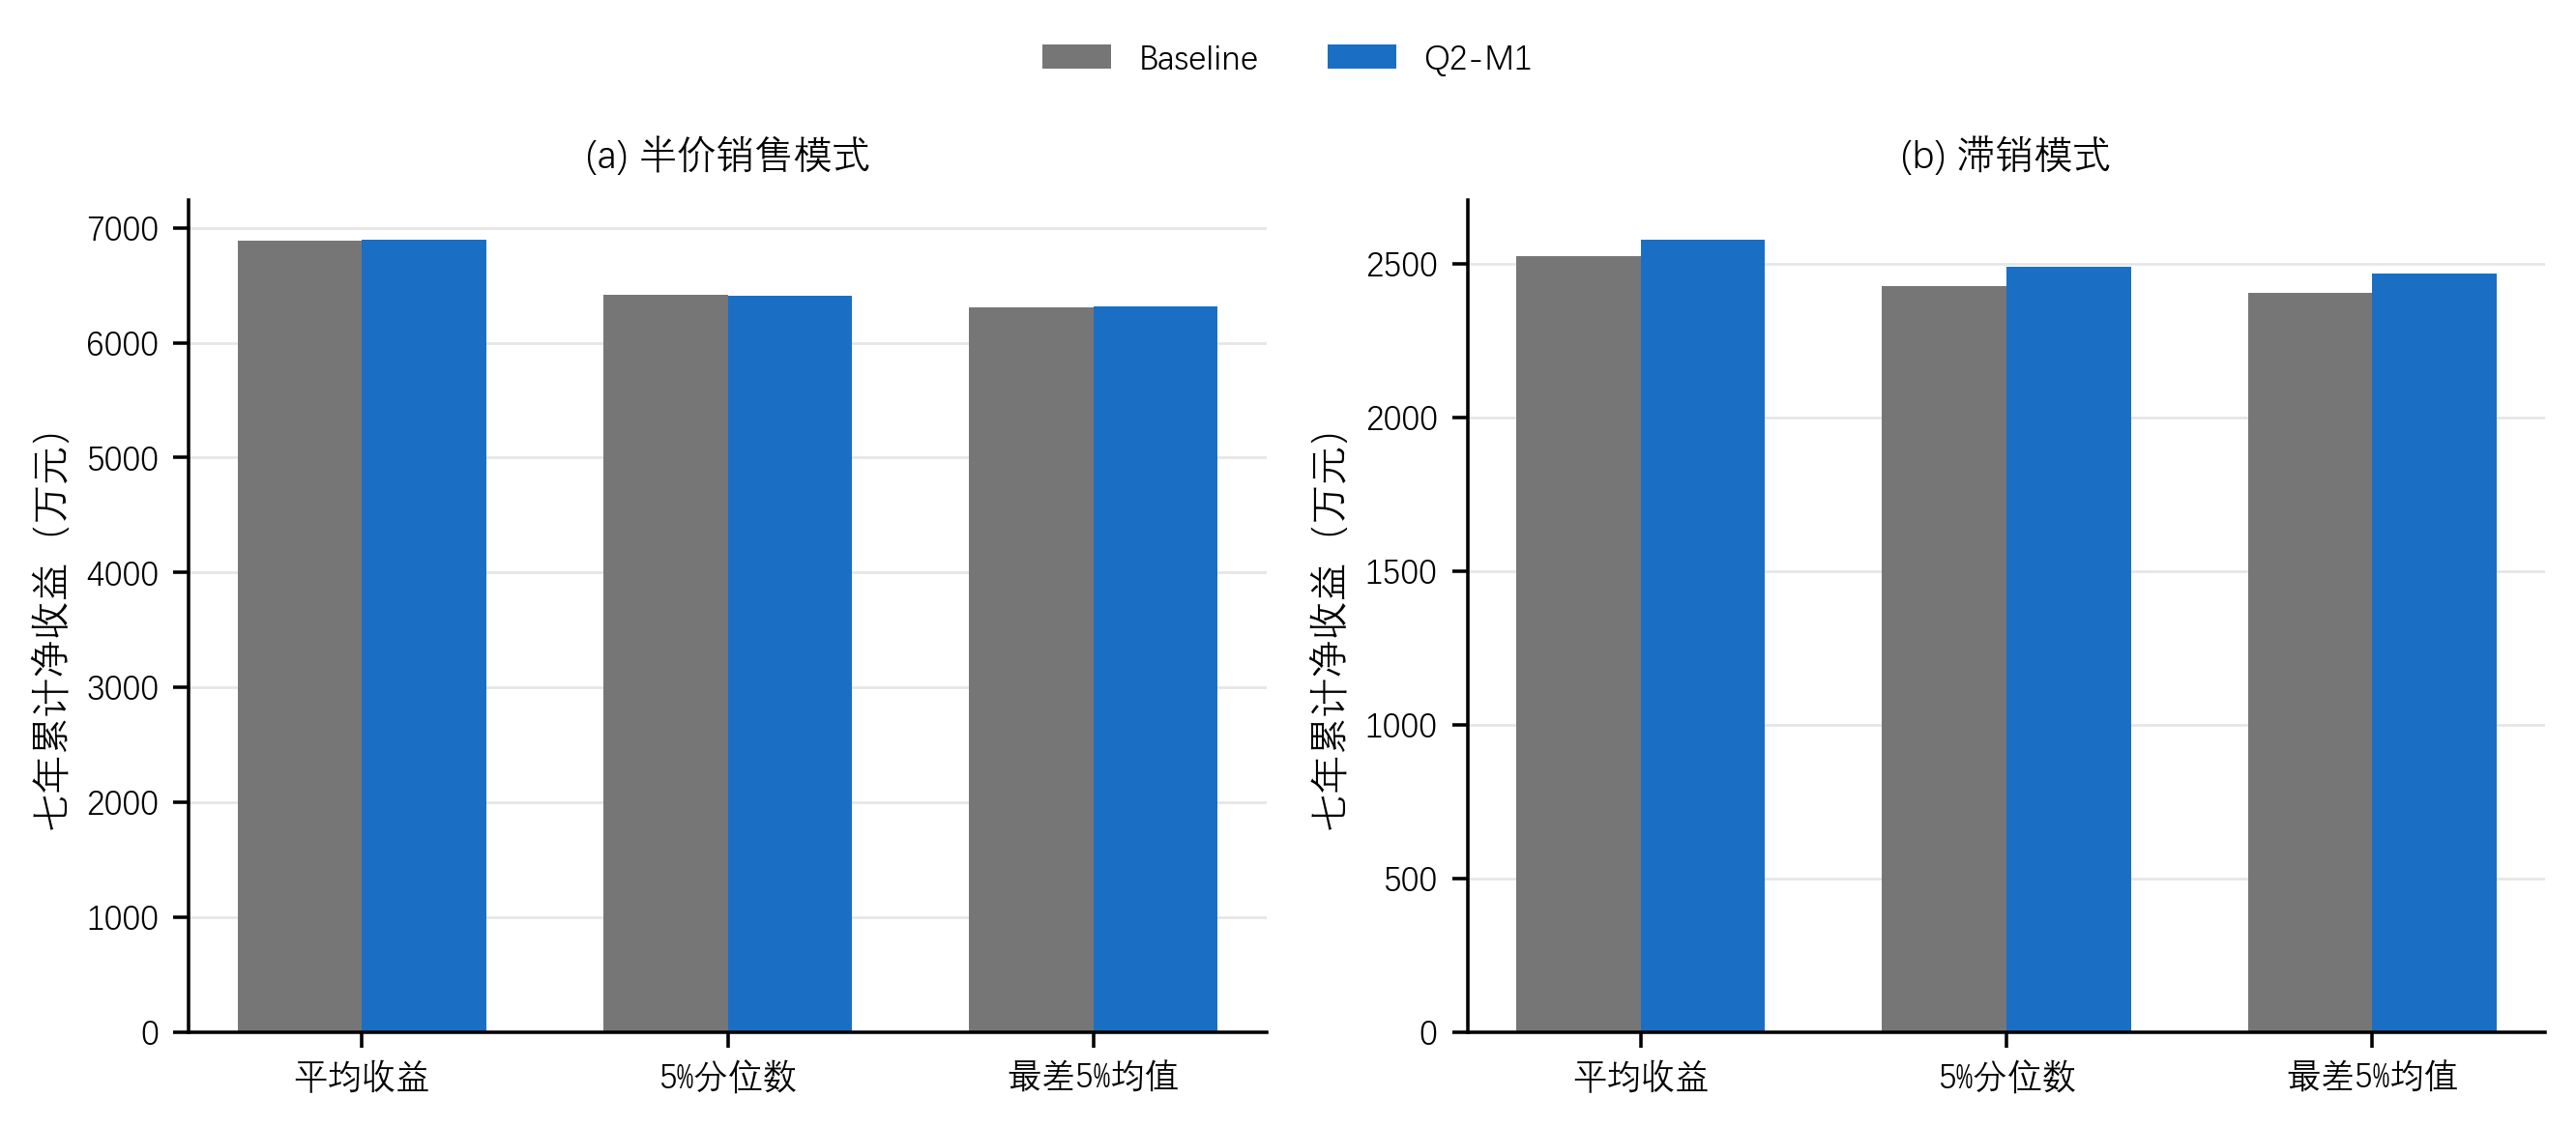
\includegraphics[width=0.96\textwidth]{figures/q2_expected_tail_comparison.png}
  \caption{问题二平均收益与下尾收益比较}
  \label{fig:q2_risk}
\end{figure}

\begin{longtable}{>{\centering\arraybackslash}p{0.13\textwidth}>{\centering\arraybackslash}p{0.11\textwidth}>{\centering\arraybackslash}p{0.15\textwidth}>{\centering\arraybackslash}p{0.15\textwidth}>{\centering\arraybackslash}p{0.15\textwidth}>{\centering\arraybackslash}p{0.13\textwidth}>{\centering\arraybackslash}p{0.08\textwidth}}
  \caption{问题二样本外风险指标}\label{tab:q2_risk}\\
  \toprule
  方法 & 模式 & 均值/万元 & 5\%分位/万元 & 下尾均值/万元 & 最低值/万元 & 亏损比例 \\
  \midrule
  \endfirsthead
  \caption{问题二样本外风险指标（续）}\\
  \toprule
  方法 & 模式 & 均值/万元 & 5\%分位/万元 & 下尾均值/万元 & 最低值/万元 & 亏损比例 \\
  \midrule
  \endhead
  \bottomrule
  \endfoot
  主方案 & 半价 & 6897.19 & 6410.00 & 6317.80 & 6192.42 & 0 \\
  基线 & 半价 & 6891.51 & 6413.87 & 6310.26 & 6184.63 & 0 \\
  主方案 & 滞销 & 2578.45 & 2489.49 & 2468.46 & 2435.22 & 0 \\
  基线 & 滞销 & 2524.71 & 2426.52 & 2405.20 & 2375.32 & 0 \\
\end{longtable}
